\clearpage
\section{Background}\label{sec-background}

Build systems automate the execution of simple repeatable tasks for individual
users, as well as for large organisations. There are software build systems,
such as \Make~\cite{feldman1979make}, \Shake~\cite{mitchell2012shake} and
\Bazel~\cite{bazel}, as well as various incremental calculation engines, such
as \Excel~\cite{advanced_excel}. In this section we use these four examples to
introduce main domain-specific notions and requirements. Other notable examples
of build systems and their relation to these four are discussed
in~\S\ref{sec-related} and~\S\ref{sec-conclusions}.

We start by giving an intuitive definition of a build system. After providing
more context and examples in the rest of this section, we
develop a formal definition in~\S\ref{sec-general-build}.

\definition[Build system]{Given a description of tasks, a \emph{build system}
executes them in an order that respects their dependencies to produce a
specified output from supplied inputs.}
\label{def-build}

\subsection{The venerable \Make: static dependencies and file modification times}
\label{sec-background-make}

\Make\footnote{There are numerous implementations of \Make and none comes with a
formal specification. In this paper we therefore use a simple and sensible
approximation to a real \Make that you might find on your machine.} was developed
more than 40 years ago to automatically build software libraries and executable
programs from source code. It uses \emph{makefiles} to describe tasks (often
referred to as \emph{build rules}) and their dependencies in a simple textual form.
For example:

\vspace{1mm}
\begin{minted}[xleftmargin=10pt]{makefile}
util.o: util.h util.c
    gcc -c util.c

main.o: util.h main.c
    gcc -c main.c

main.exe: util.o main.o
    gcc util.o main.o -o main.exe
\end{minted}
\vspace{1mm}

\noindent
The above makefile lists three tasks: (i) compile a utility library comprising
files \cmd{util.h} and \cmd{util.c} into \cmd{util.o} by
executing\footnote{In this example we pretend \cmd{gcc} is a pure function for the
sake of simplicity. In reality, there are multiple versions of \cmd{gcc} and the
actual binary that is used to compile and link files is often also listed as a task
dependency.} the command \cmd{gcc -c util.c}, (ii) compile the main source file
\cmd{main.c} into \cmd{main.o}, and (iii) link object files \cmd{util.o} and
\cmd{main.o} into the executable \cmd{main.exe}. The makefile contains the
complete information about the \emph{task dependency graph}, which is shown in
Fig.~\ref{fig-make}(a).

\begin{figure}[h]
\begin{subfigure}[b]{0.32\linewidth}
\centerline{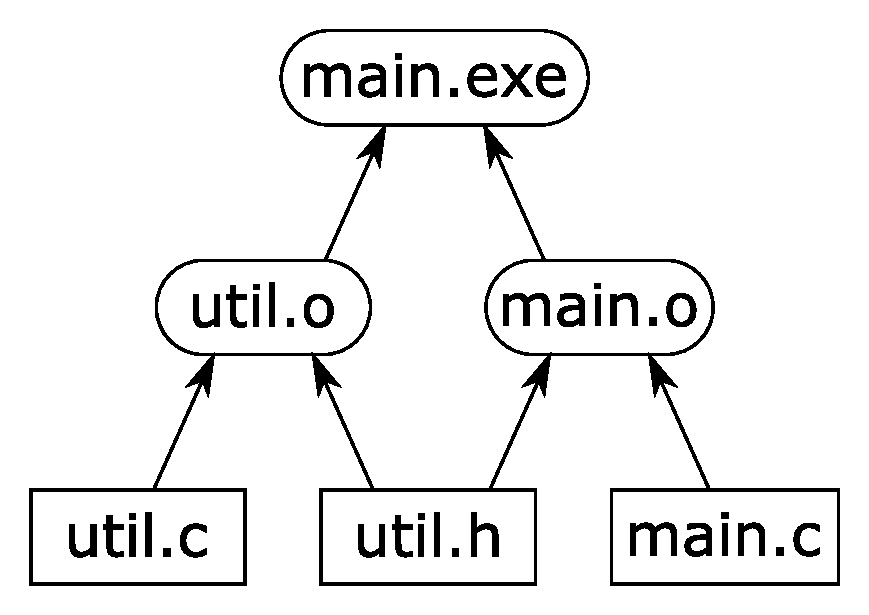
\includegraphics[scale=0.28]{fig/make-example.pdf}}
\caption{Task dependency graph}
\end{subfigure}
\begin{subfigure}[b]{0.32\linewidth}
\centerline{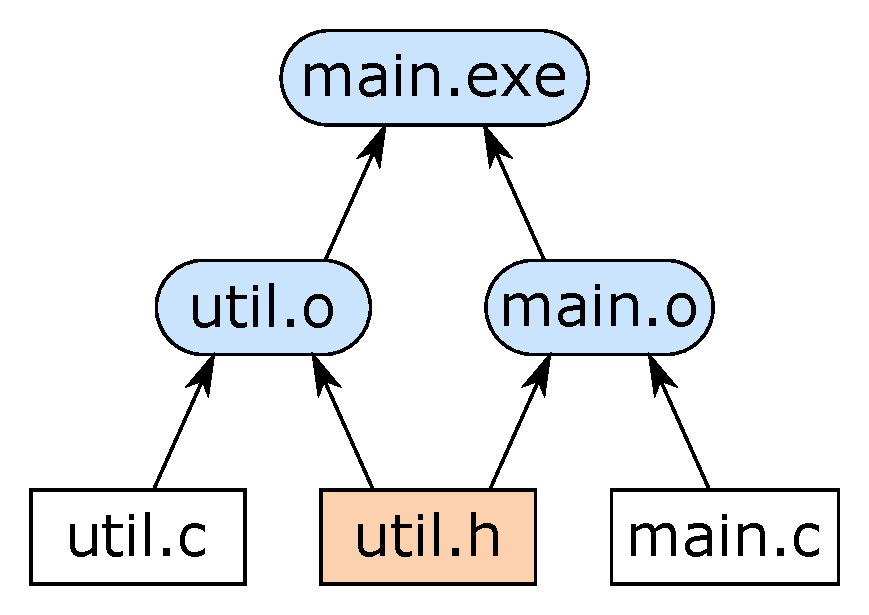
\includegraphics[scale=0.28]{fig/make-example-full.pdf}}
\caption{Full rebuild}
\end{subfigure}
\begin{subfigure}[b]{0.32\linewidth}
\centerline{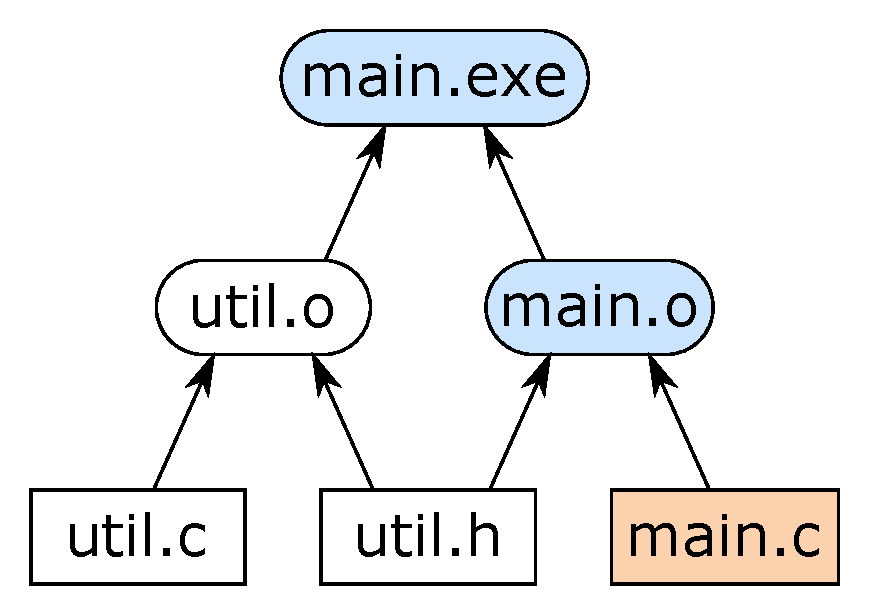
\includegraphics[scale=0.28]{fig/make-example-partial.pdf}}
\caption{Partial rebuild}
\end{subfigure}
\caption{A task dependency graph and two build scenarios. Input files are shown as
rectangles, intermediate and output files are shown as rounded rectangles. Dirty
inputs and files that are rebuilt are highlighted.
\label{fig-make}}
\end{figure}

If the user runs \Make specifying \cmd{main.exe} as the desired output, \Make
will first build \cmd{util.o} and \cmd{main.o}, in any order since the
corresponding tasks are independent, and then build \cmd{main.exe}. If the
user modifies the sources of \cmd{util.h} and runs \Make again, it will
perform a \emph{full rebuild}, because all three tasks transitively depend on
the \cmd{util.h}, as illustrated in Fig.~\ref{fig-make}(b). On the other hand, if the
user modifies \cmd{main.c} then a \emph{partial rebuild} is sufficient:
the file \cmd{util.o} does not need to be rebuilt, since its inputs have not
changed, see Fig.~\ref{fig-make}(c). Note that if the dependency graph is
\emph{acyclic} then each task needs to be executed at most once. Cyclic task
dependencies are typically not allowed in build systems although there are rare
exceptions, see~\S\ref{sec-iterative-compute}.

The following property is essential for build systems, it is their raison d'\^etre:

\definition[Minimality]{A build system is \emph{minimal} if it executes tasks at
most once per build and only if they transitively depend on inputs that changed
since the previous build.}\label{def-minimal}
\vspace{2mm}

To achieve minimality \Make relies on two main ideas: (i) it uses \emph{file
modification time} to detect which files changed\footnote{Technically, you
can fool \Make by altering the modification time of a file without changing its
content, e.g. by using the command \cmd{touch}. \Make is therefore minimal only
under the assumption that you do not do that.}, and (ii) it constructs a
complete task dependency graph from the information contained in the makefile
and executes tasks in a \emph{topological order}. For a more concrete description
see~\S\ref{sec-implementation-make}.

\subsection{\Excel: dynamic dependencies at the cost of minimality}
\label{sec-background-excel}

\Excel is a build system in disguise. Consider the following simple spreadsheet.

\vspace{1mm}
\begin{minted}[xleftmargin=10pt]{bash}
A1 = 10
A2 = 20
B1 = A1 + A2
\end{minted}
\vspace{1mm}

\noindent
There are two input cells \cmd{A1} and \cmd{A2}, and a single task that computes
the sum of their values, writing the result into the cell \cmd{B1}. If either of
the inputs change, \Excel will recompute the result.

Unlike \Make, \Excel does not need to know all task dependencies upfront. Some
dependencies may change \emph{dynamically} according to computation results. For
example:

\vspace{1mm}
\begin{minted}[xleftmargin=10pt]{bash}
A1 = 10
A2 = 20
B1 = IF(C1=1,A1,A2)
C1 = 1
\end{minted}
\vspace{1mm}

\noindent
Here the cell \cmd{C1} controls which branch of the \cmd{IF} function is used
to compute \cmd{B1}. When \cmd{C1=1}, the dependencies of \cmd{B1} are
$\{\cmd{C1},\cmd{A1}\}$, otherwise they are $\{\cmd{C1},\cmd{A2}\}$, and which is
not known statically. One might say that the value of \cmd{C1} is statically
known in this particular example, but imagine that it is the result of a long computation
chain -- its value will only become available during the build.

\Excel handles this example correctly: if \cmd{C1=1} and the user changes
\cmd{A2}, \Excel will not recompute the result \cmd{B1}. Alas, other forms of
dynamic dependencies can force \Excel to perform unnecessary computation.
Consider the following modification of the above example:

\vspace{1mm}
\begin{minted}[xleftmargin=10pt]{bash}
A1 = 10
A2 = 20
B1 = INDIRECT("A" & C1)
C1 = 1
\end{minted}
\vspace{1mm}

\noindent
The new version uses the \cmd{INDIRECT} function, which allows us to reference a
cell indirectly by a text string that is not necessarily known in advance. The
current implementation of \Excel recomputes indirect references in every
build~\cite{excel_recalc}. This clearly violates the minimality
property~\ref{def-minimal}: if \cmd{C1=1} and the user modifies \cmd{A2}, \Excel
will recompute \cmd{B1}, potentially triggering further unnecessary
recalculation even though \cmd{B1} does not transitively depend on \cmd{A2}.

\Excel's build algorithm~\cite{excel_recalc} is significantly different from
\Make. Since it is impossible to construct the full dependency graph upfront in
the presence of dynamic dependencies, \Excel uses the \emph{calculation chain}
produced by the previous build as an approximation to the correct topological
order. During recalculation, \Excel processes cells in this order, but can
\emph{defer recalculation of a cell} by moving it down the chain if a newly
discovered dependency has not yet been rebuilt. We further refer to this
algorithm as \emph{reordering}, and will discuss it in more detail
in~\S\ref{sec-implementation-excel}.

Another distinguishing feature of \Excel is \emph{self-tracking}. Most build
systems only track changes of inputs and intermediate results, but \Excel can
also track changes in the tasks themselves: if a formula is modified, \Excel
will recompute it and propagate the changes. Self-tracking is uncommon in
software build systems, where one often needs to manually initiate a full
rebuild even if just a single build task has changed. We further discuss
self-tracking in~\S\ref{sec-tracking-aspects}.

\begin{figure}[h]
\begin{subfigure}[b]{0.90\linewidth}
\centerline{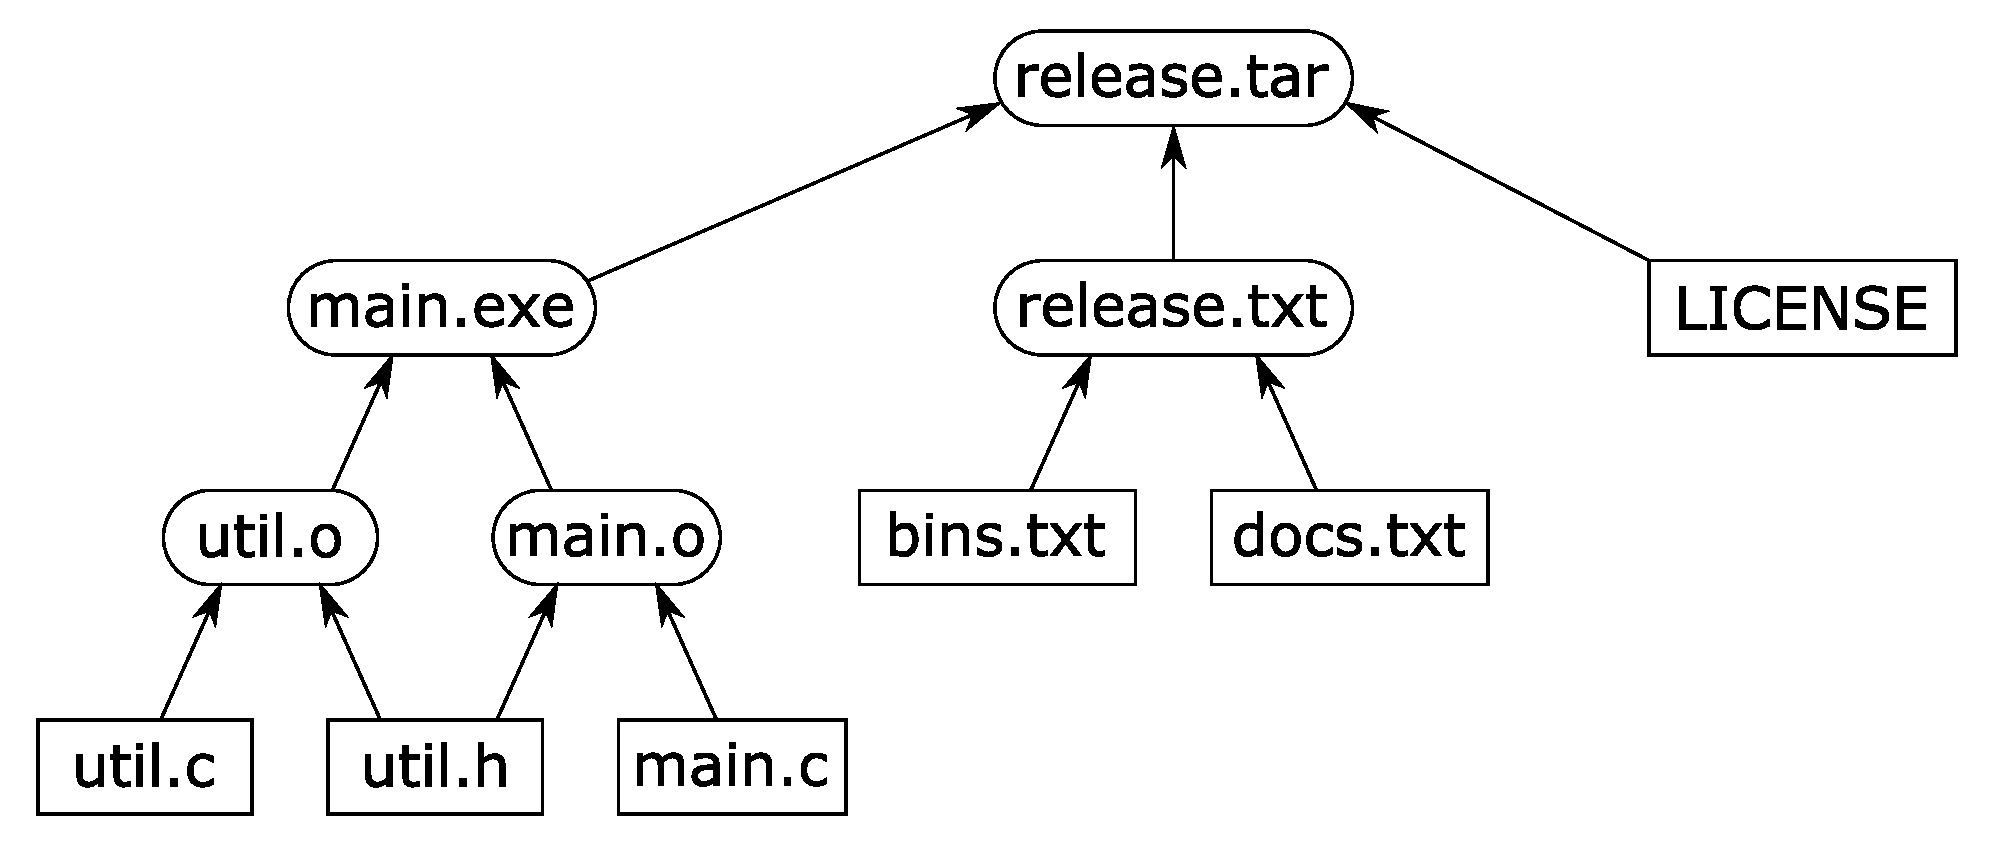
\includegraphics[scale=0.28]{fig/shake-example.pdf}}
\caption{Dependency graph produced after the previous build.}
\end{subfigure}
\begin{subfigure}[b]{0.90\linewidth}
\centerline{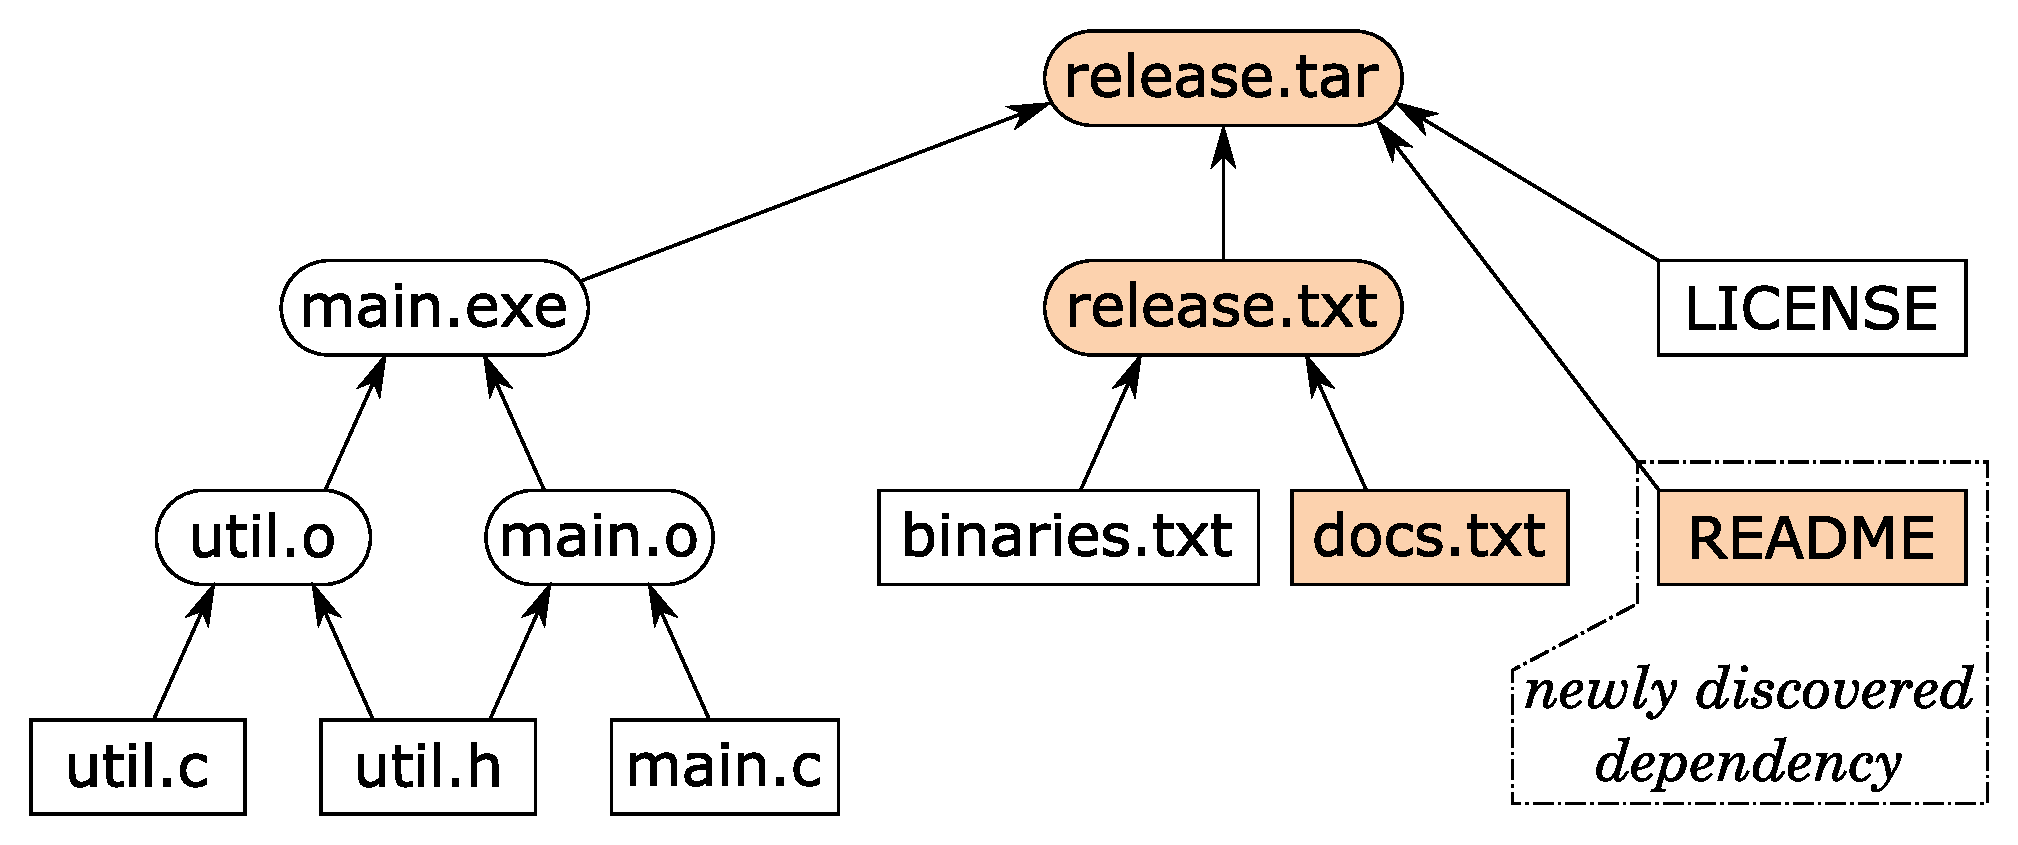
\includegraphics[scale=0.28]{fig/shake-example-rebuild.pdf}}
\caption{Since \cmd{docs.txt} has changed, we rebuild \cmd{release.txt} and
\cmd{release.tar}, discovering a new dependency.}
\end{subfigure}
\caption{Dynamic dependencies example: create \cmd{README} and add it to the
list of release documents \cmd{docs.txt}.\label{fig-shake}}
\end{figure}

\subsection{\Shake: dynamic dependencies with no remorse}
\label{sec-background-shake}

\Shake was developed to solve the issue of dynamic
dependencies~\cite{mitchell2012shake} and it excels at them without sacrificing
the minimality requirement. To demonstrate this, we elaborate the \Make example
from~\S\ref{sec-background-make} by adding the following files whose
dependencies are shown in Fig.~\ref{fig-shake}(a):

\begin{itemize}
    \item \cmd{LICENSE} is an input text file containing the project license.
    \item \cmd{release.txt} is a text file listing all release files. This file
    is produced by concatenating input files \cmd{bins.txt} and \cmd{docs.txt}
    that list all binary and documentation files of the project.
    \item \cmd{release.tar} is the release archive built by executing the
    command \cmd{tar} on the release files.
\end{itemize}

The dependencies of \cmd{release.tar} are not known statically: they are
determined by the content of \cmd{release.txt}, which might not even exist
before the build. Makefiles cannot express such dependencies, requiring ad hoc
workarounds such as \emph{build phases}, which are problematic~\cite{hadrian}.
Here is how one can express the task for producing \cmd{release.tar} using \Shake.

\vspace{1mm}
\begin{minted}[xleftmargin=10pt]{haskell}
"release.tar" %> \_ -> do
    need ["release.txt"]
    files <- lines <$> readFile "release.txt"
    need files
    system "tar" $ ["-cf", "result.tar"] ++ files
\end{minted}
\vspace{1mm}

\noindent
We first declare the static dependency on \cmd{release.txt}, then read its
content (a list of files) and depend on it, dynamically. Finally, we specify the
command to produce the resulting archive. Crucially, the archive will only be
rebuilt if one of the dependencies (static or dynamic) has changed. For example,
if we create another documentation file \cmd{README} and add it to
\cmd{docs.txt}, \Shake will appropriately rebuild \cmd{release.txt} and
\cmd{release.tar}, discovering the new dependency, as illustrated in
Fig.~\ref{fig-shake}(b).

\Shake's implementation is different from both \Make and \Excel in two aspects.
First, it uses the dependency graph from the previous build to decide which
files need to be rebuilt. This idea has a long history, going back to
\emph{incremental}~\cite{demers1981incremental},
\emph{adaptive}~\cite{acar2002adaptive}, and
\emph{self-adjusting}~\cite{acar2007selfadjusting} \emph{computations} (see a
discussion in related work~\S\ref{sec-related}). Second, instead of abandoning
and deferring the execution of tasks whose newly discovered dependencies have
not yet been built (as \Excel does), \Shake \emph{pauses} their execution until
the dependencies are brought up-to-date. We refer to this build algorithm as
\emph{recursive}.

\begin{figure}[h]
\centerline{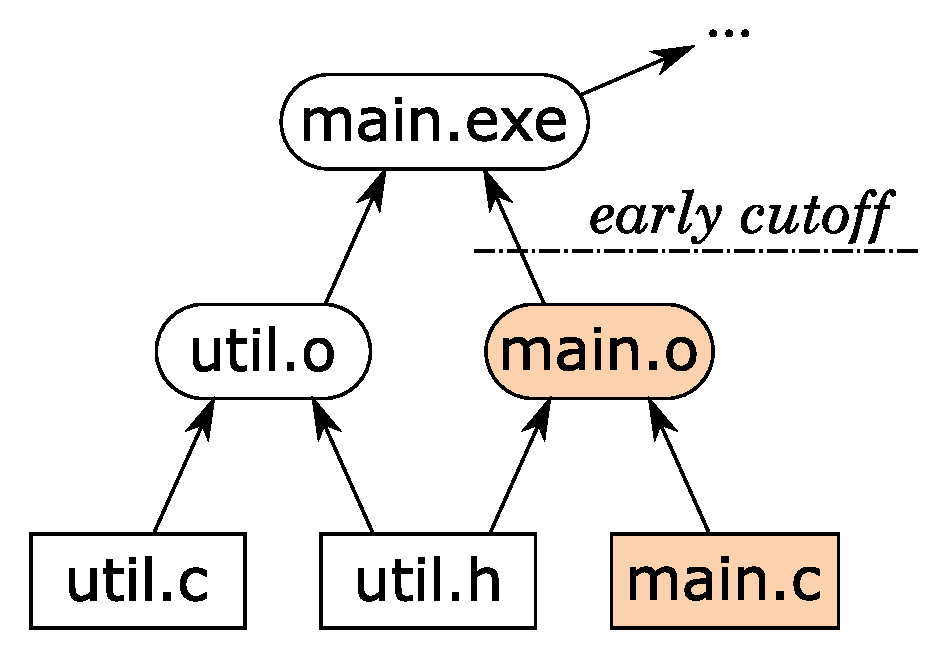
\includegraphics[scale=0.28]{fig/shake-example-cutoff.pdf}}
\vspace{-2mm}
\caption{An early cutoff example: if a comment is added to \cmd{main.c}, the
rebuild is stopped after detecting that \cmd{main.o} is unchanged, since this
indicates that \cmd{main.exe} and its dependents do not need to be
rebuilt.\label{fig-cutoff}}
\end{figure}

\Shake also supports the following \emph{early cutoff optimisation}. When it
executes a task and the result is unchanged from the previous build, it is
unnecessary to execute the dependent tasks, and hence \Shake can stop a build
earlier, as illustrated in Fig.~\ref{fig-cutoff}. Not all build systems support
early cutoff: \Make and \Excel do not, whereas \Shake and \Bazel (introduced
below) do.

\subsection{\Bazel: a cloud build system}
\label{sec-background-bazel}

When build systems are used by large teams, different team members
often end up executing exactly the same tasks on their local machines.
A \emph{cloud build system} can speed up builds dramatically by
transparently sharing build results among team members. Furthermore, cloud
build systems allow one to perform \emph{shallow builds} that materialise
only end build products on a local machine, leaving all intermediates in the
cloud. This is a significant optimisation compared to \emph{deep builds}
that require all transitive dependencies of an end build product to be
locally available. % Non-cloud build systems cannot support shallow builds.

\Bazel is one of the first examples of openly available cloud build systems.
Like \Make, it does not support dynamic dependencies and can therefore benefit
from the simplicity of building tasks in a statically known topological order.
It is minimal and supports the early cutoff optimisation.

To support cloud builds, \Bazel maintains a conventional \emph{content-addressable
cache}, which can be used to fetch a previously built file given the hash of its
content, as well as \emph{dependency graphs from all previous builds}, annotated
with observed file hashes\footnote{Here we ignore the issue of limited cloud
storage resources for the sake of simplicity; in practice, old entries are
regularly evicted from the storage, as further discussed
in~\S\ref{sec-cloud-aspects}.}. The latter allows to bypass the execution of
a task, by predicting the hash of the result from the hashes of its dependencies,
and subsequently fetching the result from the cache. A concrete implementation is
provided in~\S\ref{sec-implementations}.

\subsection{Summary}
\label{sec-background-summary}

We summarise differences between four discussed build systems in
Table~\ref{tab-summary}. The `Metadata' column refers to the \emph{auxiliary
build information} persistently stored between builds by all build systems:
\begin{itemize}
    \item \Make stores file modification times, or rather, it relies on the file
    system to do that. In principle a single \emph{dirty bit} per file is
    sufficient, as will be demonstrated in~\S\ref{sec-implementations}.
    \item \Excel stores one dirty bit per cell and the calculation chain from
    the previous build.
    \item \Shake stores the dependency graph discovered in the previous build,
    annotated with file content hashes for efficient checking of file changes.
    \item \Bazel stores all dependency graphs discovered in previous builds
    annotated with file hashes, and the content-addressable cache.
\end{itemize}

\begin{table}[h]
\smaller
\centering
\begin{tabular}{l||l|l||l|c|c|c}
\hline
$\!$Build system$\!$& Metadata                       & Algorithm    & Dependencies & Minimal & Cutoff & Cloud$\!$\\\hline
$\!$\Make       $\!$& File modification times        & Topological  & Static       & Yes     & No     & No   $\!$\\
$\!$\Excel      $\!$& Dirty cells, calculation chain & Reordering   & Dynamic      & No      & No     & No   $\!$\\
$\!$\Shake      $\!$& Previous dependency graph      & Recursive    & Dynamic      & Yes     & Yes    & No   $\!$\\
$\!$\Bazel      $\!$& All dependency graphs, cache   & Topological  & Static       & Yes     & Yes    & Yes  $\!$\\\hline
\hline
\end{tabular}
\vspace{2mm}
\caption{Summary of build system differences.\label{tab-summary}}
\vspace{-7mm}
\end{table}

In this paper we elucidate which build system properties are consequences of
specific implementation choices (metadata and algorithm), and how one can obtain
new build systems with desired properties by recombining parts of existing
implementations. As a compelling example, we demonstrate how to combine
advantages of \Shake and \Bazel in a cloud build system with dynamic
dependencies, see~\S\ref{sec-implementation-cloud-shake}.
